\chapter[Search for top squarks in all-hadronic final states]{Search for top squarks in all-hadronic final states}
\label{ch:stop_ana}
\epigraph{\emph{In God we trust. All others must bring data.}}{William E. Deming}

	In this chapter the core of this thesis will be presented, namely the search for the direct pair-production of the supersymmetric partner of the top quark in all-hadronic final states using \pp\ collisions, at a centre-of-mass energy $\rts = 13$ \TeV, delivered by the \ac{LHC} and collected by the \ac{ATLAS} detector. A dataset of $36.1\, \ifb$ was used. Such measured value of integrated luminosity has an uncertainty of 3.2\% based on studies of scans of the $x-y$ beam separation carried out on both $2015$ and $2016$ datasets, where the average pileup parameter $\mu$ was $13.7$ and $24.9$, respectively.
		
	The results produced were published in a paper in the Journal of High Energy Physics in September 2017~\cite{stop0L}. A previous version of the analysis was also made public, using $13.3\,\ifb$ collected at $\rts = 13$ \TeV, with an earlier subset of the whole $2015+2016$ dataset, documented in an ATLAS conference note~\cite{ICHEPstop0L}. Although both versions contain author's contributions, only the results of the most recent analysis will be hereby discussed, as it represents the most updated, improved and extended version. Specifically, the optimisation of the search strategy, as well as the data-driven estimation of the number of events in the search regions for one of the most important backgrounds, and the evaluation of the related theory uncertainties, characterised the author's contributions. In addition, exception made for the optimisation strategy, the same contributions were also used in a different \ac{SUSY} analysis published in October 2017 in~\cite{DMhf}. Further details can be found in Appendix~\ref{ch:appA}.

	The chapter will be structured as it follows: an excursus on the simplified \ac{SUSY} models considered will be presented in Section~\ref{sec:susysig}; the selection of the events and the objects used in both data and \ac{MC} will be presented in Section~\ref{sec:evtsel}; the variables used and the optimisation of the regions in which the \ac{SUSY} signals were searched for will be presented in Section~\ref{sec:SRs}; the nominal procedure used  for the background estimation will be discussed in Section~\ref{sec:bkgest}, with particular focus on the data-driven background estimation in Section~\ref{sec:ddbkgest}; the results, together with their interpretation, will finally be presented in Section~\ref{sec:results}.


	\section{SUSY Signals}
	\label{sec:susysig}

		As already introduced in Section~\ref{sec:SUSYPheno}, the signals considered in this work are generated using simplified models, meaning that only the \stop, the \ninoone, the \ninotwo, and the \chinoonepm, were the \ac{SUSY} particles considered. In particular, in such considered models, either \ninotwo\ or \chinoonepm\ is assumed to be the \ac{NLSP} and, the chargino-neutralino mass splitting $\Delta m(\chinoonepm, \ninoone)$ is assumed to be $1$ \GeV, in accordance with the naturalness argument. This implies that the \chinoonepm\ will promptly decay to $\Wboson^*\ninoone$ , with the \Wboson\ emitted as a virtual particle. The decay products of the so-created virtual \Wboson\ will therefore be low \pt\ objects which will not be reconstructed by the \ac{ATLAS} detector. 

		\subsection{Benchmark processes}

			\begin{figure}[!htb]
				% \begin{center}
				\centering
					\subbottom[$\stop\ra t^{(*)}\ninoone$]{
						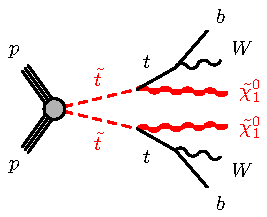
\includegraphics[width=0.25\textwidth]{theory/stst-bqqbqqN1N1-tt}}\hspace{0.05\textwidth}
					\subbottom[$\stop\ra b\ \chinoonepm\ra b \Wboson^{(*)}\ninoone$]{
						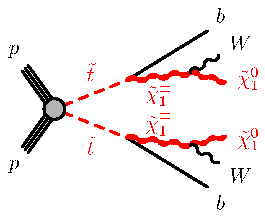
\includegraphics[width=0.25\textwidth]{theory/stst-bbWWN1N1}}\hspace{0.05\textwidth}
					\subbottom[$\stop\ra t\ \ninotwo\to h/Z\ \ninoone$]{
						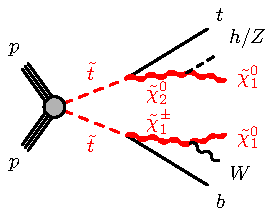
\includegraphics[width=0.25\textwidth]{theory/stst-tbhWN1N1}}\hspace{0.05\textwidth}
				% \end{center}
				\caption{Diagrams of the decay topologies of the signal models considered in this work.}
				\label{fig:stopModels}
			\end{figure}

			Figure~\ref{fig:stopModels}(a)$-$(c) shows the diagrams corresponding to the decay scenarios considered in this work. In particular, (a) where both top squarks decay\footnote{The symbol (*) indicates off-shell production} via $\stop\rightarrow t^{(*)}\ \ninoone$; (b) where at least one of the stops decays via $\stop\rightarrow b\ \chinoonepm \rightarrow b\ \Wboson^{(*)}\ \ninoone$; (c) where $m_{\ninotwo}$ is small enough to allow one stop to decay via $\stop\to t\ \ninotwo \to h/Z\ \ninoone$ where $h$ is the \ac{SM} Higgs boson;

			\begin{wrapfigure}{R}{.5\textwidth}
				\centering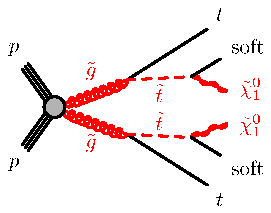
\includegraphics[width=.25\textwidth]{theory/gogo-tsofttsoftN1N1-stst}
				\caption{Diagram of the gluino-mediated top squark production. The term ``soft" refers to decay products whose transverse momenta are below the detector thresholds.}
				\label{fig:gtt}
			\end{wrapfigure}

			The results were interpreted in the simplified models where only one- and two-step decays scenarios are allowed and, as already mentioned, the latter will be referred to as a natural \ac{SUSY}-inspired mixed grid, \ie\ $\Delta m(\chinoonepm, \ninoone) = 1 \GeV$~\cite{Alwall:2008ve, Alwall:2008ag, Alves:2011wf}. Furthermore, in both scenarios the \ac{LSP} is considered to be a pure bino state. The results will also be interpreted in two slices of the \ac{pMSSM} models: wino-\ac{NLSP} and well-tempered neutralino \ac{pMSSM}~\cite{Djouadi:1998di, Berger:2008cq}.
			A fourth scenario, in addition to direct pair production, was considered: top squarks can also be indirectly produced via gluino decays, as illustrated in Figure~\ref{fig:gtt}. In such model, the mass difference between the top squark and the neutralino is considered to be relatively small, $\Delta m(\stopone, \ninoone) = 5$ \GeV, allowing the jets originating from \stopone\ decay to have a \pt\ below the reconstruction threshold of the \ac{ATLAS} detector resulting in an experimental signature nearly equivalent to the one in Figure~\ref{fig:stopModels}(a).


		\subsection{MC samples}

			A grid of points across the $(\mstopone-\mninoone)$ plane with a $50$-\GeV\ spacing is generated to simulate the above-mentioned simplified models. %The mixing between the partners of the left- and right-handed top quarks is assumed to be maximal, \ie\ ..
			The signal models were generated using \texttt{MG5\_aMC@NLO 2.2-2.4}~\cite{madgraph} interfaced to \texttt{PYTHIA8}~\cite{pythia8} for the \ac{PS} and hadronisation. \texttt{EvtGen 1.2.0}~\cite{evtGen} was employed for the decays of the  $b$- and $c$-hadrons. The tree-level \ac{ME} calculation includes the emission of up to two additional partons for all signal samples. The \texttt{NNPDF2.3LO} \ac{PDF}~\cite{PDFs} set was used to generate the signal samples with the \texttt{A14}~\cite{CT10} tune for the \ac{UE} and shower parameters. Additionally, the CKKW-L prescription~\cite{CKKW} was used for the \ac{ME}–\ac{PS} matching. 

			The various signal cross sections were all calculated to next-to-leading order in the strong coupling constant, with the addition of soft-gluon emission re-summation at next-to-leading-logarithm accuracy (NLO+NLL)~\cite{Beenakker:1997ut, Beenakker:2010nq, Beenakker:2011fu}. The sparticle mass spectra for \ac{pMSSM} models were calculated using \texttt{Softsusy 3.7.3}~\cite{Allanach:2001kg, Allanach:2013kza} while the decays of each sparticle were performed by \texttt{HDECAY 3.4}~\cite{hdecay} and \texttt{SDECAY 1.5/1.5a}~\cite{sdecay}. Finally, various \ac{PDF} sets, factorisation, and re-normalisation scales were used to generate an envelope of cross-section predictions, within which a nominal value and uncertainty were chosen. Further details can be found in~\cite{Borschensky:2014cia}.



	\section{Objects definition}
	\label{sec:obj_def}
			
		The physics objects, as output of the reconstruction algorithms discussed in Section~\ref{sec:objReco}, are required to pass a first loose selection to be categorised as \emph{baseline} objects. An additional procedure is employed, to remove potentially overlapping objects, \eg\ a lepton is identified as a jet, or a lepton that falls within the same jet cone. The so-called \ac{OR} procedure, whose inputs are two baseline objects, is employed to resolve such ambiguity by discarding on of the two objects by looking at their $\Delta R$ as shown in Table~\ref{tab:OR}. 

		\begin{table}[!htb]\centering\caption{List of the possible ambiguities with relative criteria and decisions.}
			\begin{tabular}{cccc}
				\toprule 
				\textbf{Ambiguity} & \textbf{Criterion} & \textbf{Object kept} & \textbf{Object removed}\\
				\toprule
				\multirow{2}{*}{electron/jet} & $\Delta R (e,\mathrm{jet}) < 0.2$ & electron & jet\\
				& $0.2 \leq \Delta R (e,\mathrm{jet}) < 0.4$ & jet & electron \\\midrule
				electron/\bj & $\Delta R (e,\bj) < 0.2$ & \bj\ & electron\\ \midrule
				\multirow{2}{*}{muon/jet} & $\Delta R (\mu,\mathrm{jet}) < 0.4$ and & \multirow{2}{*}{muon} & \multirow{2}{*}{jet} \\ 
						& $N_{\mathrm{tracks}} < 3$, $\pt^{\mathrm{track}} > 500$ \MeV &  &  \\ \midrule
				photon/electron & $\Delta R (e,\gamma) < 0.4$ & electron & photon\\ 
				photon/muon & $\Delta R (\mu,\gamma) < 0.4$ & muon & photon\\ 
				photon/jet & $\Delta R (\mathrm{jet}, \gamma) < 0.4$ & jet & photon\\ 
				\bottomrule
				\end{tabular}
				\label{tab:OR}
		\end{table}

		The data-driven estimation of \ttZ\ events using \ttgamma\ is the only part of the analysis that used reconstructed photons. In particular, the \ac{OR} is modified accordingly to avoid that an object will appear in multiple collections (double-counting). The various baseline and signal objects can now be defined as it follows:

		\begin{description}
			\item[Electrons] 
				baseline electrons are required to have $\abseta < 2.47$, $\pT > 7$ \GeV\ and have to pass a variant of the \texttt{VeryLoose} likelihood-based selection (further details in~\cite{egamma, egamma2}). Electron candidates which pass the \ac{OR}, have a $\pt > 20$ \gev\ ($\pt > 28$ \GeV) in regions with a \met\ (lepton) trigger, satisfy $d_0/\sigma_{d_{0}} < 5$, $z_0 \sin \theta < 0.5$, and pass a \texttt{Tight} likelihood-based selection isolation, are tagged as signal;

			\item[Muons] 	
				baseline muons have to pass a \texttt{Loose} selection~\cite{PERF-2015-10}, satisfy $\abseta < 2.7$ and $\pt > 6$ \GeV. Further requirements are imposed on muon candidates to tag them as signal. In particular, they have to pass the \ac{OR}, a \texttt{Medium} quality selection~\cite{PERF-2015-10}, and satisfy
				$|d_0|< 3 \sigma_{d_0}$ and $|z_0 \times \sin \theta |<0.5$. Additionally, the \pt\ requirement is tightened up to $20$ \gev\ ($28$ \GeV) in regions with a \met\ (lepton) trigger;

			\item[Photons]
				baseline photons have to pass a \texttt{Tight}~\cite{Aaboud:2016yuq} selection, and have $\pt > 25$ \GeV\ and $\abseta < 2.37$. Additionally, baseline photon candidates are required to have $\pt > 130$ \GeV\ and satisfy a tighter isolation selection, in order to be tagged as signal;
			
			\item[Jets]
				as already mentioned in Chapter~\ref{sec:objReco}, jets are reconstructed using the \antikt\ algorithm with $R=0.4$. Baseline jets are required to have $\pt>20$ \GeV\ and $\abseta< 4.8$. Signal jets have to pass the \ac{OR}, satisfy the \ac{JVT} requirement, and have $\abseta < 2.8$ and $\pt > 20$ \GeV. 

			\item[b-tagged jets]
				baseline jets in the event are identified as originating from the decay of a $b$-quark is based on the \texttt{MV2c10} jet tagger which uses the a $77\%$ fixed-cut WP. The \pt\ threshold applied to signal jets is also applied to \bj\ and the requirement on the pseudorapidity is relaxed down to $\abseta < 2.5$.
			
			\item[Missing transverse energy]
				The \met\ is reconstructed as described in Section~\ref{sec:objReco}. Baseline muons, electrons, and jets after overlap removal are used in the \met\ recalculation. 
				% The \textit{soft} term in the event, already introduced in Section~\ref{sec:objReco}, that is not associated with any of the selected objects is calculated from inner detector tracks with $\pt > 400$ \MeV\ matched to the \ac{PV} to make it more resilient to pileup contaminations. 

				Additionally, in the analysis carried out during Run-1~\cite{Atlas8TeV} another \met-related quantity was introduced. The track-based \met, derived from the sum of the \pt\ of the tracks associated with the objects in the event was found to have discriminating power to reject fake \met. The \ptmisstrk, whose magnitude is \mettrk, from the tracking system is computed using the vector sum of the reconstructed inner detector tracks, $\ptmisstrk = \sum_i^{\mathrm{tracks}} \pt^i$, with $\pT > 500$ \MeV\ and $\abseta < 2.5$, that are associated with the \ac{PV} in the event. 
 		\end{description}

		Ultimately, leptons are also required to satisfy \pt-dependent track- and calorimeter-based isolation criteria. The calorimeter-based isolation is determined by taking the ratio of the sum of energy deposits in a cone of $R = 0.2$ around the electron or muon candidate and the energy deposits associated with the electron and muon. The track-based isolation is estimated in a similar way but using a variable cone size with a maximum value of $R = 0.2$ for electrons and $R = 0.3$ for muons. An isolation requirement is made that is $95\%$ efficient for electron or muon candidates with $\pt = 25$ \GeV\ and $99\%$ for candidates with $\pt = 60$ \GeV.


	\section{Event Selection}
	\label{sec:evtsel}

		The \ac{ATLAS} detector did not operate with the same conditions during $2015$ and $2016$, meaning that different triggers and objects (calibration parameters) were used. In order for \ac{MC} parameters to be modified consistently with what is done in data, \ac{MC} events are assigned a random number, which identifies an ATLAS run. This allows \ac{MC} events to be associated with specific data-taking periods such that their parameters are associated what is done in data and can be modified accordingly.

		\subsection*{Triggers}

			As previously discussed at the end of Chapters~\ref{ch:detector} and in Chapter~\ref{ch:trigger}, physics events are recorded once they passed a certain trigger. In particular, a \met\ trigger is used to select events that fall in signal-enriched regions, \ac{SR}, where $0$ leptons ($\ell$) are required; a single-lepton (photon) trigger is used for background-enriched regions, where $1$-lepton (photon) is required. A breakdown of all the lowest unprescaled online triggers used will be presented below;

			\begin{description}
				\item [Missing transverse energy] once the \met\ is reconstructed from an input jet collection, a $70$-\GeV\ threshold is required in the $2015$ dataset whereas, due to the increase in instantaneous luminosity (impact on the trigger rate), in $2016$ the threshold was gradually raised to $90$, $100$, and $110$ \GeV. It can be seen (Figure~\ref{fig:mettrigger}) that for analysis purposes a cut of at least $200$ \GeV\ is required to stay in a region where the trigger is fully efficient (\emph{plateau}); 

				\item [Single electron] events with an electron are triggered on using a logic \texttt{OR} of three chains. In particular, the first consists of a $24$-\GeV\ ($26$-\GeV) threshold, together with an \ac{L1} isolation, in $2015$ ($2016$) data; the second chain uses a $60$-\GeV\ threshold without additional isolation requirement; the third uses a $120$-\GeV\ threshold to be efficient at high \et; a $\pt^e > 27$ \GeV\ cut is applied to stay in the plateau region;

				\item [Single muon] a logic \texttt{OR} of two chains is instead used to trigger events with muons; a first chain with a $20$-\GeV\ threshold is used in data $2015$ and $26$-\GeV\ threshold, together with an isolation requirement, in $2016$; a second chain with a $50$-\GeV\ threshold is employed for both $2015$ and $2016$ data; a $\pt^\mu > 27$ \GeV\ is applied to stay in the plateau region;

				\item [Single photon] unlike the lepton case, only one chain is used to select events with photons; a $120$ \GeV\ ($140$ \GeV) threshold is employed in $2015$ ($2016$). Additionally, in order to ensure full trigger efficiency a $\pt^\gamma > 150$ \GeV\ cut is applied.
			\end{description}


		\subsection*{Event cleaning}

			In order to remove events where the a detector fault occurred, a set of offline cuts is applied. The first requirement for an event to be a good physics event, is the existence of a primary vertex with a minimum of two tracks, with $\pt\ > 400$ \MeV, associated with it. Once this is passed, the status of both \ac{ECAL} and \ac{HCAL} for that event is checked: if any of the calorimeters returned an error state, the event is discarded. In addition, to reduce and suppress the fake-jet contamination a \emph{bad jet} requirement is defined by introducing quality requirements on a variety of jet parameters, \eg\ the fraction of energy deposited in the different layers of the calorimeters, and the fraction of jet \pt\ measured by the tracks in the Inner Detector. Events containing bad jets that passed the \ac{OR} are discarded. Similarly, events containing baseline muon candidates, whose relative uncertainty on $e/p$ is larger than $20\%$, and which were found before the \ac{OR}, are discarded. This also applies to events containing those potentially cosmic muons which were not removed by the \ac{OR}.	


	\section{Signal Regions}
	\label{sec:SRs}

		

	% 	\subsection{Variables used}

	% 	\subsection{Optimisation}


	% \section{Nominal Background Estimation}
	% \label{sec:bkgest}

	% 	\subsection{Control Regions}

	% 	\subsection{Validation Regions}


	% \section{Data-Driven Background Estimation}
	% \label{sec:ddbkgest}


	% \section{Results and Interpretation}
	% \label{sec:results}
